% The dvipsnames option is passed to the xcolor package, which beamer loads
\documentclass[xcolor={dvipsnames}]{beamer}

\usepackage{smpa2152-style}

\title[Data Ethics]{Data Ethics}
\author[SMPA 2152]{Data Analysis for Journalism and Political Communication (Fall 2025)}
\date{Prof. Bell}

\begin{document}

%%%%%%%%%%%%%%%%%%%%%%%%%%%%%%%%%%%%%%%%%%%%%%%%%%%%%%%%%%%%%%%%%%
\frame{
\titlepage
}

%%%%%%%%%%%%%%%%%%%%%%%%%%%%%%%%%%%%%%%%%%%%%%%%%%%%%%%%%%%%%%%%%%
\frame{\frametitle{Tuskegee Syphilis Study}
\centering
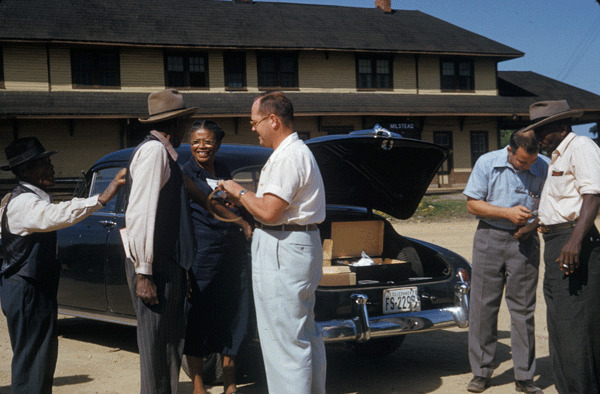
\includegraphics[width=.8\textwidth]{tuskegee}
}

%%%%%%%%%%%%%%%%%%%%%%%%%%%%%%%%%%%%%%%%%%%%%%%%%%%%%%%%%%%%%%%%%%
\frame{\frametitle{The Belmont Report (1978)}
\only<1-2>{
    \begin{itemize}[<+->]
        \item Summarizes ethical principles and guidelines for conducting research with human subjects
        \item Codified into law as the ``Common Rule'', which covers all federally-funded research
    \end{itemize}
}
\only<3->{
\begin{block}{Respect for Persons}
    Individuals should be treated as autonomous agents, and persons with diminished autonomy are entitled to protection.
\end{block}
}
\vfill
\only<4->{
\begin{block}{Beneficence}
     (1) Do not harm and (2) maximize possible benefits and minimize possible harms.
\end{block}
}
\vfill
\only<5>{
\begin{block}{Justice}
     Groups who bear the burden of research should also be the beneficiaries of that research.
\end{block}
}
}

%%%%%%%%%%%%%%%%%%%%%%%%%%%%%%%%%%%%%%%%%%%%%%%%%%%%%%%%%%%%%%%%%%
\frame{\frametitle{Other Considerations}
\begin{itemize}[<+->]
    \item Informed Consent
    \begin{itemize}
        \item<.-> Subjects must affirmatively agree to participate in research
        \item Participants must have all information necessary to make an informed decision
        \item What about studies that require deception? Studies that compensate participants?
    \end{itemize}
    \item Weighing benefits and risks of research
    \begin{itemize}
        \item<.-> Is there a way to gain the information sought in the study that minimizes risk?
        \item If risks cannot be reduced, how great is the potential benefit to society and to the subject?
        \item Examples: Stanford Prison Experiment, \href{https://www.youtube.com/watch?v=Kzd6Ew3TraA}{Milgram Experiment}
        \item[] vs. randomized drug trials
    \end{itemize}
\end{itemize}

}

%%%%%%%%%%%%%%%%%%%%%%%%%%%%%%%%%%%%%%%%%%%%%%%%%%%%%%%%%%%%%%%%%%
\frame{\frametitle{Expanding Principles for Equity (Urban Institute)}

\begin{itemize}
    \item Seek and include communities' interests in
research design
    \item Seek out and incorporate communities' interpretation of the data
    \item Return data and research results to community
members in a form they can use
    \item Be aware of how sensitive topics can affect
people and communities
    \item Minimize the amount of personally identifiable
information (PII) collected
    \item Avoid undue burden
    \item Share data to reduce the burden of duplicate
data collection
\end{itemize}

}

%%%%%%%%%%%%%%%%%%%%%%%%%%%%%%%%%%%%%%%%%%%%%%%%%%%%%%%%%%%%%%%%%%
\frame{\frametitle{Example: Project Nightingale}

In 2019, the \textit{Wall Street Journal} reported that the nation's second-largest health care provider, Ascension, provided Google with access to tens of millions of health records to develop AI tools that ``make health records more useful, more accessible, and more searchable.''

\begin{itemize}[<+(1)->]
    \item There was no informed consent from patients
    \item There is potential harm from the release of health records
    \item Google claims that the data was sufficiently protected and staff properly trained
    \item Improving health care is a general societal good
    \item Because there is no ``opt-in,'' the data is not biased in favor of certain demographic groups
    \item There are financial benefits that accrue to the companies, not the research subjects
\end{itemize}
}

%%%%%%%%%%%%%%%%%%%%%%%%%%%%%%%%%%%%%%%%%%%%%%%%%%%%%%%%%%%%%%%%%%
\frame{\frametitle{Case Studies}
\large
\only<1>{
\begin{enumerate}
    \item Home DNA Testing
    \item Crisis Text Line
    \item Diversity in Faces (DiF) dataset
\end{enumerate}
}
\only<2>{
\small
\begin{enumerate}
    \setlength{\itemsep}{0pt} % Reduces space to zero
    \item What are the relevant ethical principles and practices?
    \item What concerns are there about violations of ethical principles?
    \item How could the research have been conducted more ethically?
\end{enumerate}
\inserttimer{8}
}
}

%%%%%%%%%%%%%%%%%%%%%%%%%%%%%%%%%%%%%%%%%%%%%%%%%%%%%%%%%%%%%%%%%%
\frame{\frametitle{De-identification}
\begin{itemize}[<+->]
    \item Researchers often promise \textbf{\textit{anonymity}} or \textbf{\textit{confidentiality}} to participants in order to reduce the risks of participating in research
    \item There are two types of identifiers that must be removed before sharing this data:
    \begin{enumerate}
        \item \textbf{Direct identifiers}: information that would be sufficient on its own to disclose an identity, such as names, addresses, and phone numbers.
        \item \textbf{Indirect identifiers}: information that \textit{in combination} would be sufficient to disclose an identity
    \end{enumerate}
    \item De-identification is the process of removing direct and indirect identifiers
\end{itemize}
}

%%%%%%%%%%%%%%%%%%%%%%%%%%%%%%%%%%%%%%%%%%%%%%%%%%%%%%%%%%%%%%%%%%
\frame{\frametitle{De-identification}

\begin{enumerate}[<+->]
    \item Remove direct identifiers
    \item Aggregate or reduce the precision of a variable
    \begin{itemize}
        \item<.-> Generalize the meaning of categories
        \item Collapse categories
        \item Restrict the upper or lower ranges
    \end{itemize}
    \item Anonymize keys that link to other datasets
    \item Maintain a master log of all replacements, aggregations, or removals and keep it in a secure location separate from the de-identified data files
\end{enumerate}

\only<1>{
\centering
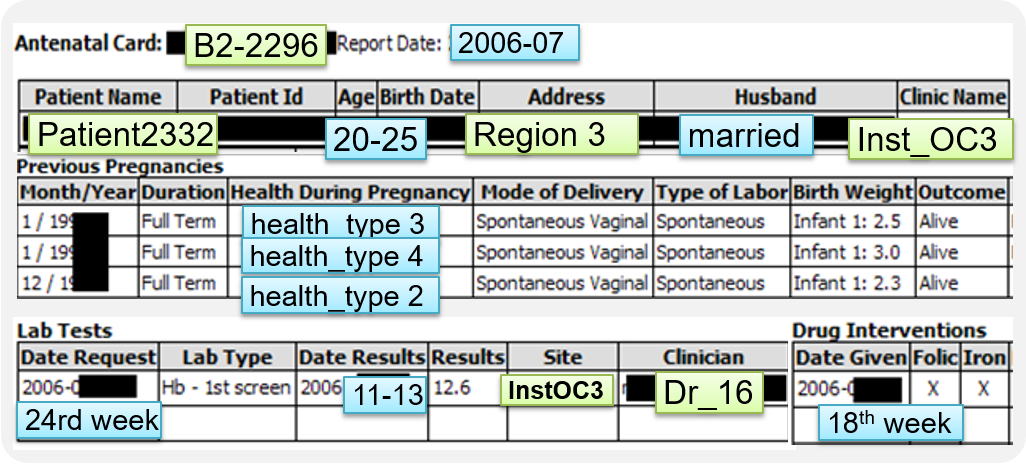
\includegraphics[height=.33\textheight]{remove_direct_identifiers.png}
}
\only<2>{
\centering
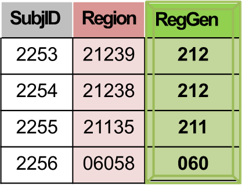
\includegraphics[height=.33\textheight]{generalize_categories.png}
}
\only<3>{
\centering
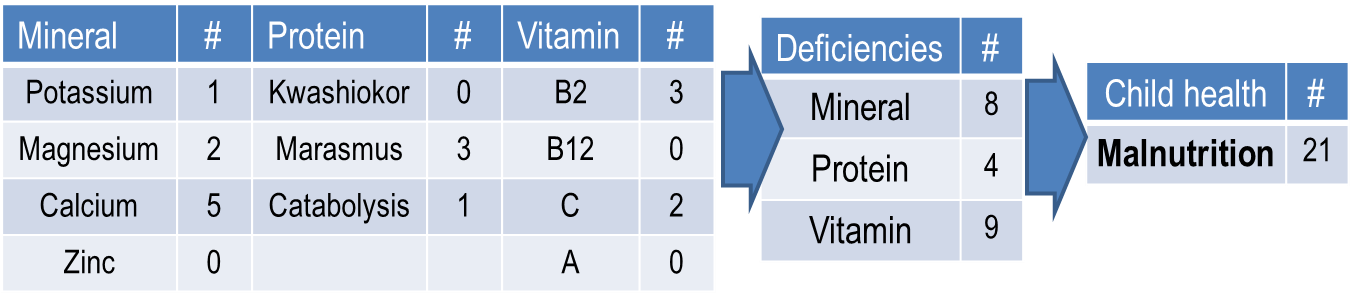
\includegraphics[height=.25\textheight]{collapse_categories.png}
}
\only<4>{
\centering
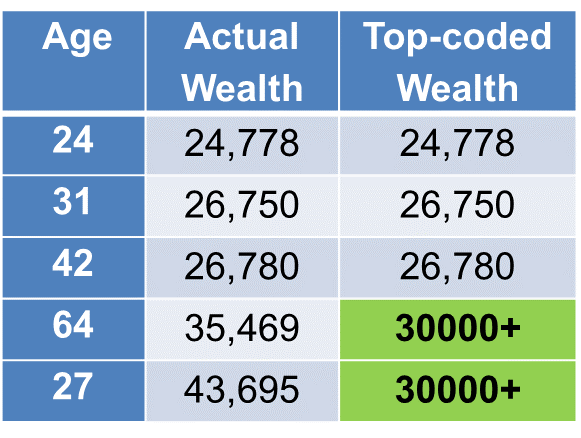
\includegraphics[height=.33\textheight]{top-code.png}
}
\only<5->{
~\\
\centering
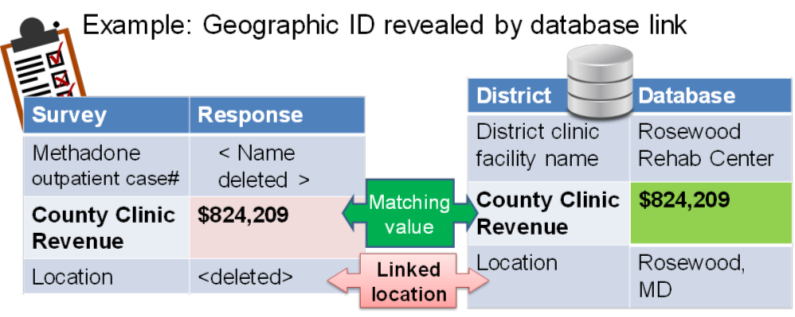
\includegraphics[height=.33\textheight]{remove_relational_links.png}
}
}

%%%%%%%%%%%%%%%%%%%%%%%%%%%%%%%%%%%%%%%%%%%%%%%%%%%%%%%%%%%%%%%%%%
\frame{\frametitle{De-identification Exercise}
\inserttimer{8}
}

\end{document}
